% ============================================================
% ch5_discussion.tex -- 第五章：討論、多層規劃議程與研究限制
% 譯自 paper/en/back.tex 第 6--8 節（Integrative Discussion, MLP Agenda, Limitations）。
% 所有數字取自 raw_materials/experimental_log.md；多層規劃模型常數為
% raw_materials/idea.md 之 v1.0 正式規格。治理型態 C／F／D 不得展開為任何名稱。
% ============================================================

\chapter{討論、多層規劃議程與研究限制}
\label{zh:ch:discussion}

\section{綜合討論}
\label{zh:sec:discussion}

\subsection{三條資料線共同顯示的結果}
\label{zh:sec:discussion_lines}

在三條資料線中，唯有專利資料提供了具外部指派群體標籤之行動者之間的有向二元流動，而這正是中介（brokerage）分析所需要的資料 \citep{gould1989structures}；研究一的引用資料線原則上可能承載此類流動，但因資料與設計上的原因而未能達成（第~\ref{zh:sec:study1_network}~節），且沒有任何公開資料來源通過流動效度關卡（表~\ref{zh:tab:app_sources}）。三項專利分析共用同一資料來源，並非彼此獨立的複製研究。

綜合來看，這些資料線支持以下四項陳述。第一，在領域層次上，依本研究之定義，AI 與決策技術呈現過度連結（over-connection），而非彼此分隔，且此結果在各種設定下皆穩健；此過度連結正在下降，儘管其預先登錄（preregistration）標籤為 \texttt{PERSISTENT}（第~\ref{zh:sec:study2_aggregate}~節；圖~\ref{zh:fig:patent_trend}），且在排除 G06Q10/04 以及採用粒度匹配的參照集時，判定仍然成立（表~\ref{zh:tab:construct}；第~\ref{zh:sec:lim_measurement}~節）。第二，在此一過度連結的領域配對之內，格層次的偏低大多幅度有限，且無法在前後兩半時期中複製（第~\ref{zh:sec:study2_suite}~節；圖~\ref{zh:fig:cpc_heatmap}）。第三，在公司層次上，超出專利組合構成所能解釋的部分之外，仍存在顯著的專門型公司（specialist firm）分隔（分別佔與 1 之差距的 15\% 與 9\%；以比值尺度衡量則短缺 33\% 與 22\%），而混合型（多角化）公司（mixed-portfolio firm）是否對此分隔進行中介，則仍未解決（第~\ref{zh:sec:study2_firm}~節；圖~\ref{zh:fig:firm_null}）。第四，沒有任何資料線證實 Burt 意義上的結構洞（structural hole）：研究一的網路資料線找到 0 個經證實的中介者（HISTORICAL / USER\_REPORTED），而 CORDIS 二分網路（bipartite network）虛無模型（null model）則找到 0 個顯著候選者。

這些結果看似與研究一相互矛盾：在研究一中，全部 16 個偏低的功能配對在兩個時期皆維持偏低。然而兩者涉及不同的分析單位與參照基準。研究一探討的是哪些「功能配對」在文件中共現（co-occurrence），其參照為一個封閉之 $10\times12$ 矩陣的邊際；由於期望次數的總和等於觀察總數，部分格的偏低必然意味著其他格的偏高（核心格中兩者各有 16 個）。偏低格（depleted cell）描述的是既有連結的「組成」，而非其「數量」。研究二探討的則是兩個「技術領域」彼此交換引用的強度，其參照為 179 個可比較的領域。兩者的持續性判準亦不相同——研究一僅看方向，專利研究則要求三項檢定在前後兩半時期皆顯著（其中一半樣本較小）——因此兩者的對比並非同類比較。在兩條資料線中，格層次的發現皆為一個相互連結之整體內部的相對偏離，而非分隔的證據。綜合而言，證據並不支持 AI 與決策技術之間的知識流動（knowledge flow）存在結構洞（RQ1）。在公司層次（RQ2），結構洞既未獲證實，亦未被排除：判定結果為 \texttt{PARTIAL}，且目前沒有任何可用的虛無模型能同時固定度數與專利組合。本研究不主張任何因果效果。

\subsection{對缺口研究的測量啟示}
\label{zh:sec:discussion_measurement}

本研究計畫記錄了共現資料與隸屬（affiliation）資料的四種失效模式，每一種皆有直接證據。\textbf{投影派系（projection cliques）：}CORDIS 共同成員關係的投影會人為製造封閉性（第~\ref{zh:sec:theory_cooccurrence}~節），而在投影之後計算的中介並非二模中介 \citep{jasny2015two}。\textbf{限制度在二分網路中的退化：}在嚴格的二分網路中，網路限制度（network constraint）會退化為二元集中度——而批評者早已指出，這正是主導該指標的成分 \citep{everett2020unpacking,johnson2026reassessing}。這是一個恆等關係；而在 120 格中有 104 格具觀察值的矩陣中，或在一個稠密的 $6\times7$ 矩陣中，每一個偏低格周圍都能找到替代路徑幾乎是必然的；這些缺口效度（Gap Validity）檢查是對資料結構的診斷，而非關於這些領域的證據。\textbf{同詞兩端共用}（same-term self-pairing）與\textbf{模型推論標籤}（model-inferred labels）（第~\ref{zh:sec:study1_direction}~節與第~\ref{zh:sec:study1_reliability}~節）屬於非隨機誤差。隨機、非差異性的誤分類（misclassification, non-differential）只會削弱偏低，但在邊際固定的矩陣中，膨脹某一格會機械性地使其所在列與欄的其餘部分偏低。在研究一中，此機制並非主要驅動因素：排除同詞紀錄後，13/16 個偏低格維持其方向，而移除同詞兩端共用的紀錄僅使核心格減少 2 格。模型推論標籤仍是一個未經檢驗的非隨機誤差來源，因此該方向僅屬描述性，且未獲證實。結構洞測度在不同資料類型之間無法互換 \citep{saglietto2020research}；這四種機制具體說明了其原因。前兩者為已知結果；本研究計畫補充的是它們對缺口推論的影響。

有兩項啟示涉及虛無模型。第一，當每份文件皆貢獻一個完整的列 $\times$ 欄區塊時，保留文件結構的交換虛無模型（M06）會退化；M06-P（專利適用之保留文件結構虛無模型）雖保留了該結構，但未經型一錯誤校準（第~\ref{zh:sec:study2_cells}~節）。第二，公司限制度的解讀取決於虛無模型固定了什麼：相對於度數配對的標籤置換虛無模型，混合型公司看似具有較低的限制度（$p=.001$）；相對於保留專利組合的虛無模型（portfolio-preserving null），其限制度則高於預期（$p=1.000$）。前一個虛無模型忽略了公司擁有什麼，後一個則忽略了公司有多少連結；用於檢驗中介的虛無模型必須同時固定兩者。

由此可得三項設計上的啟示。檢定應採相對比較，因為跨領域的 O/E 低於 1 乃是常態。決策規則應在檢視真實資料之前先以合成資料加以校準，且所用的生成器應比本研究所用者更不簡化。規則、停止規則（stop rule）與修訂（amendment）應事先固定並據實報告（表~\ref{zh:tab:app_prereg} 與表~\ref{zh:tab:app_amend}），且最好透過第三方登錄平台為之。對缺口研究而言，實務意涵很簡單：偏低格並不等於缺口；低限制度的節點也不是中介者，除非它能通過一個同時保留專利組合與度數的虛無模型的檢驗。

\subsection{負面結果尚未釐清之處}
\label{zh:sec:discussion_hypothesis}

本研究所檢驗的前提，是本研究計畫自身由共現證據所導出的工作前提。未能找到知識流動上的結構洞，並不證明結構洞不存在，但它移除了將 AI 與決策之整合視為一個「橋接問題」的一項理由。它既未確立困難所在，也未使任何單一替代解釋變得更為可能：研究一與研究二不含任何組織內部資料，而專利公司網路所記錄的是受讓人（assignee）之間的引用，而非公司如何部署 AI。至少有五項候選解釋仍屬未決，而本研究的資料對其中任何一項皆無直接的證據力。(1)~\textbf{組織資源分配（resource allocation）與決策權（decision rights）：}預算、核准鏈與治理規則允許或禁止 AI 的特定用途，並規範人類與 AI 在決策中如何配置。(2)~\textbf{資料品質：}流程所需的資料缺漏、品質不佳或未經整合。(3)~\textbf{成本：}整合可行且獲得允許，但其預期價值不足以支應其成本。(4)~\textbf{法規與責任：}外部規則或責任歸屬要求由人類做出決策，或禁止自動化。(5)~\textbf{任務適配性：}AI 在該任務上表現不佳，或該任務具有不確定性或多義性，而有利於人類判斷 \citep{jarrahi2018artificial}；不同的決策任務條件有利於不同的人機結構 \citep{shrestha2019organizational}。這些解釋並非互斥，且其中數項可能同時在同一家公司中產生約束。

組織層面的候選解釋，正是本研究計畫之模型所表徵的那一項。它借鑑了「經濟行動鑲嵌於具體、持續之關係中」的觀點 \citep{granovetter1985economic}，以及第~\ref{zh:sec:intro}~章所回顧的管理文獻 \citep{shrestha2019organizational,raisch2021artificial,berente2021managing}；這些文獻為模型的層級設計提供了動機，但既未檢驗該模型，也未使其優於其他候選解釋。究竟是哪一項候選解釋在組織內部或外部產生約束，正是研究三設計來加以區辨的問題（第~\ref{zh:sec:mlp_study3}~節）。

% ------------------------------------------------------------
\section{多層規劃研究議程}
\label{zh:sec:mlp}

本節是負面結果的後續延伸，而非由該結果推得的結論。它僅將第~\ref{zh:sec:discussion_hypothesis}~節中的組織候選解釋加以形式化；該解釋涉及不同行動者之間的巢狀決策：企業分配資源，架構與治理層決定 AI 整合與受監督的深度，而流程負責人則選擇人機配置，且每一方皆預期其下層行動者的回應。這正是多層規劃（multi-level programming, MLP）的結構：領導者（leader）在追隨者（follower）之最適回應的限制下進行最佳化 \citep{dempe2002foundations,colson2007overview}。

\subsection{形式模型}
\label{zh:sec:mlp_model}

令 $i\in I$ 為決策流程的索引，$r\in\{D,A,R,G\}$ 為能力資源（資料、AI、可靠性與治理）的索引，每項資源皆以順序尺度 $\{0,1,2,3\}$ 衡量；$\kappa_i$ 為流程的後果等級（與 Cohen's $\kappa$ 無關）。企業的預算為 $B_{\mathrm{tot}}$，並在治理型態（governance regime）$\Gamma\in\{C,F,D\}$ 下運作；在原型中，治理型態僅是一組參數：容量 $K_\Gamma$、風險、成本與彈性的乘數，以及許可矩陣 $\mathrm{Allow}_{m\Gamma}$（表~\ref{zh:tab:app_regimes}）。正式的 v1.0 模型共有三層，其完整陳述見附錄~\ref{zh:app:mlp_full}：
\begin{itemize}
\item \textbf{第一層（領導者）}在預算內分配整數資源 $b_i^r$，以提高能力上限 $\bar D_i,\bar A_i,\bar R_i,\bar G_i$，並最大化 $F_1$；$F_1$ 為已實現價值與 AI 採用數的加權和，減去資源使用量與剩餘風險，各項皆於追隨者的回應下評估。
\item \textbf{第二層}為每個流程選擇 AI 整合深度 $A_i$、人類監督 $H_i$、工作流程整合 $WI_i$ 與保證 $EA_i$，以最大化 $F_2$；其限制條件包括能力上限、隨 $A_i$ 與 $\kappa_i$ 提高的要求門檻（表~\ref{zh:tab:app_thresholds}），以及由所有流程共用的治理容量 $K_\Gamma$。附錄~\ref{zh:app:mlp} 列出 $F_2$ 及其組成項，以及其未經校準的設計權重（式~\eqref{zh:eq:app_f2}）。
\item \textbf{第三層（追隨者）：}每個流程選擇一種獲許可的配置——\texttt{HumanOnly}、\texttt{AIAssist}、\texttt{HumanFirstAICheck}、\texttt{AIFirstReview} 或 \texttt{BoundedAutomation}——其最低第二層要求從 \texttt{HumanOnly} 的「無要求」逐步提高至 \texttt{BoundedAutomation} 的最高要求（表~\ref{zh:tab:app_configs}）。
\end{itemize}
在選擇型流程中，固定的分數門檻 $\tau_i$ 決定 AI 的建議（式~\eqref{zh:eq:mlp_tau}）；它是一種敏感度分析工具，而非錯誤率的模型。

\paragraph{性質、範圍與錨定。}在五項假設下，所選定的三層解組合存在，且窮舉式逆向歸納必然終止（附錄~\ref{zh:app:mlp}）；對此一有界原型進行精確窮舉，並不構成可處理性（tractability）的主張 \citep{jeroslow1985polynomial}。v1.0 原先作為門檻錨定的研究一 16 個 V9 偏低格已予撤回：它們並非經驗上已驗證的缺口，且其方向未獲證實（第~\ref{zh:sec:discussion_measurement}~節）。每一項門檻、權重與許可皆為設計假設，唯有在組織候選解釋通過研究三的檢驗時，才會在研究三中加以校準。

\subsection{模擬示例}
\label{zh:sec:mlp_sim}

所有係數皆為模擬值，輸出結果不描述任何真實公司。表~\ref{zh:tab:back_mlp_scenarios} 與圖~\ref{zh:fig:mlp_scenarios} 報告九個基準情境（三個流程；治理型態 C、F 與 D；預算 3、5 與 7；所有配置皆獲許可），以精確逆向歸納求解；針對 768 個案例所進行的一致性檢查發現，與正式限制式之間的不一致為 0 件（附錄~\ref{zh:app:mlp}）。

\begin{table}[tbp]
\centering
\caption{三層原型之模擬基準情境（SIMULATED；無公司資料）。治理型態僅為參數集合（表~\ref{zh:tab:app_regimes}）。}
\label{zh:tab:back_mlp_scenarios}
\small
\setlength{\tabcolsep}{4pt}
\begin{tabular}{lrrrrrl}
\toprule
治理型態 & 預算 & $F_1$ & \begin{tabular}[b]{@{}r@{}}實現\\價值\end{tabular} & \begin{tabular}[b]{@{}r@{}}剩餘\\風險\end{tabular} & \begin{tabular}[b]{@{}r@{}}AI\\採用數\end{tabular} & 配置（三個流程） \\
\midrule
C & 3 & 1.708 & 1.560 & 0.268 & 2 & \texttt{AIAssist} $\times2$，\texttt{HumanOnly} $\times1$ \\
F & 3 & 1.775 & 1.642 & 0.316 & 2 & \texttt{AIAssist} $\times2$，\texttt{HumanOnly} $\times1$ \\
D & 3 & 1.842 & 1.724 & 0.363 & 2 & \texttt{AIAssist} $\times2$，\texttt{HumanOnly} $\times1$ \\
\midrule
C & 5 & 2.158 & 2.221 & 0.451 & 3 & \texttt{AIAssist} $\times3$ \\
F & 5 & 2.244 & 2.338 & 0.530 & 3 & \texttt{AIAssist} $\times3$ \\
D & 5 & 2.331 & 2.454 & 0.610 & 3 & \texttt{AIAssist} $\times3$ \\
\midrule
C & 7 & 2.158 & 2.221 & 0.451 & 3 & \texttt{AIAssist} $\times3$（與預算 5 相同） \\
F & 7 & 2.244 & 2.338 & 0.530 & 3 & \texttt{AIAssist} $\times3$（與預算 5 相同） \\
D & 7 & 2.616 & 3.286 & 0.736 & 3 & \texttt{AIAssist} $\times2$，\texttt{HumanFirstAICheck} $\times1$ \\
\bottomrule
\end{tabular}
\end{table}

\begin{figure}[tbp]
\centering
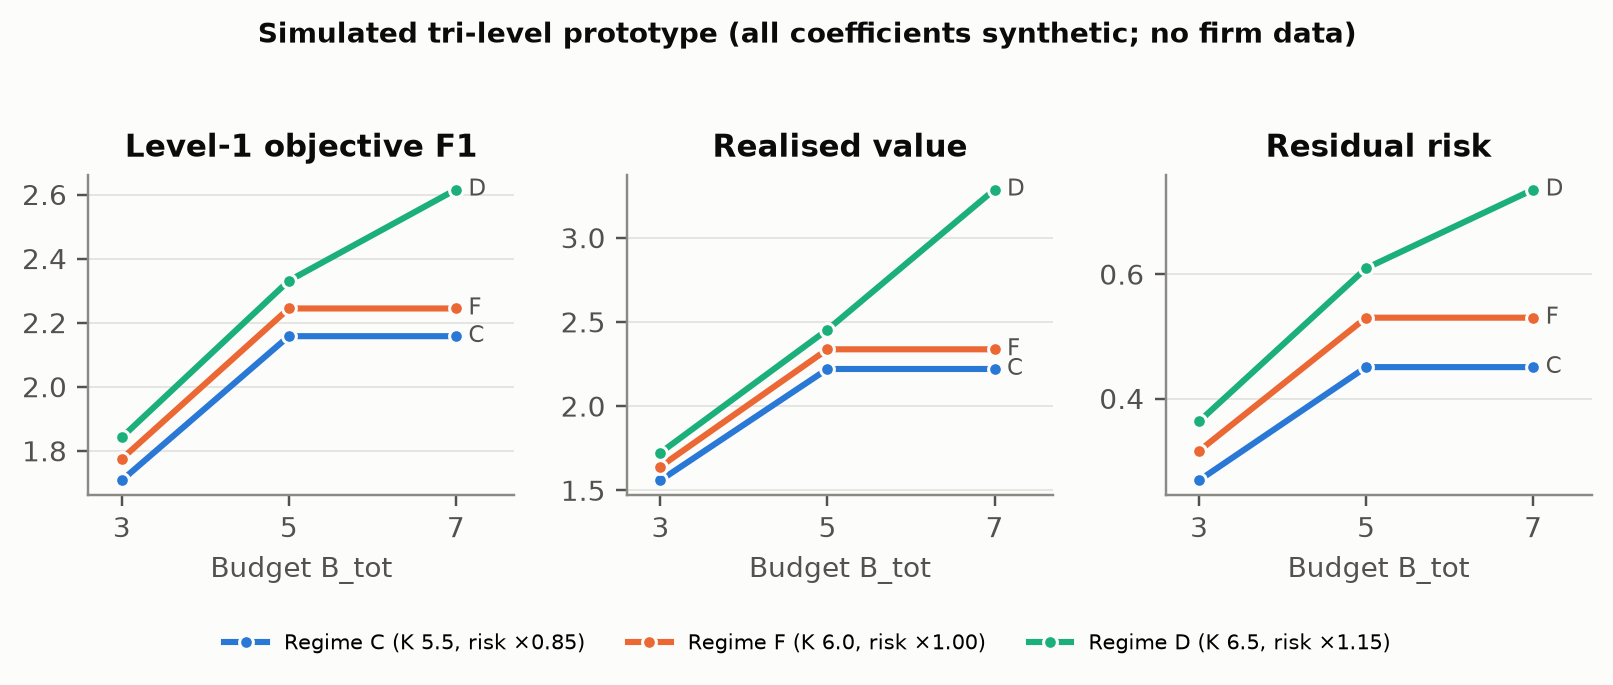
\includegraphics[width=\linewidth]{fig_mlp_scenarios.png}
\caption{模擬之三層原型：在預算 $B_{\mathrm{tot}}\in\{3,5,7\}$ 下，治理型態 C（$K$ 5.5，風險 $\times0.85$）、F（$K$ 6.0，風險 $\times1.00$）與 D（$K$ 6.5，風險 $\times1.15$）的第一層目標 $F_1$、實現價值與剩餘風險。所有係數皆為模擬值；未使用任何公司資料，輸出結果亦不描述任何真實公司。在 C 與 F 之下，預算 7 的解與預算 5 的解相同；在 D 之下，預算 7 時有一個流程改採 \texttt{HumanFirstAICheck}。}
\label{zh:fig:mlp_scenarios}
\end{figure}

此模式是機械性的：在每一預算水準內，$F_1$、實現價值與剩餘風險皆依 C、F、D 的順序遞增，這反映的是治理型態的參數設定，而非組織的任何特性。

兩項探測僅用以說明模型機制，而非研究發現。在「治理許可探測」（治理型態 C，預算 5）中，\texttt{AIAssist} 被禁止：$F_1$ 從 2.158 降至 0.837，配置則從 \texttt{AIAssist} $\times3$ 變為 \texttt{HumanOnly} $\times2$ 加上 \texttt{HumanFirstAICheck} $\times1$。治理型態與預算皆未改變，但第一層會重新最佳化其分配，因此能力是內生的，而非保持固定。此一轉變在建構上即由許可所驅動，因為移除最適配置會迫使模型改採次一順位的可行配置；研究三必須在資料中觀察到此類模式。在「選擇門檻探測」（治理型態 F，預算 5）中，流程 P2 的分數為 0.65，真實結果為 1。當 $\tau\leq0.6$ 時，P2 採用 \texttt{AIAssist}（$F_1$ 2.244，即 F/5 基準）；當 $\tau=0.7$ 時，AI 的建議錯誤，第一層不再分配任何資源給 P2 的 AI 能力，P2 因而退回 \texttt{HumanOnly}（$F_1$ 1.450）。由於分數與結果固定且為各層所知，此探測對錯誤率不具任何意涵。

\subsection{研究三：預先登錄之企業研究（計畫，而非結果）}
\label{zh:sec:mlp_study3}

研究三依序有兩個目標：其一是在第~\ref{zh:sec:discussion_hypothesis}~節的五項候選解釋之間加以區辨；其二是唯有在組織候選解釋獲得支持時，才對模型進行校準。目前尚未蒐集任何資料。

\paragraph{競爭解釋（competing explanations）及其特徵。}各候選解釋的差異在於：將 AI 整合進某一決策流程的嘗試會在「何處」停止，以及必須改變「什麼」才能使其繼續推進（表~\ref{zh:tab:back_study3_rivals}）。所有特徵皆為觀察性的。當可行且獲許可的配置因其整合成本即使在重新分配後仍超出預算而遭拒絕時，即為成本構成約束；當總體上存在預算、但領導者將其分配至他處，或內部決策權阻擋採用時，則為分配構成約束。內部決策權與外部法規的差別，在於構成約束的規則源自公司內部或外部。

\begin{table}[tbp]
\centering
\caption{研究三（計畫）：候選解釋、其在模型中的對應項，以及各自在整合事件中所預測的觀察特徵。目前尚未蒐集任何資料。}
\label{zh:tab:back_study3_rivals}
\footnotesize
\begin{tabular}{p{3.0cm}p{3.2cm}p{8.0cm}}
\toprule
候選解釋 & 模型對應項 & 預測特徵 \tabularnewline
\midrule
\raggedright 組織分配與決策權 & \raggedright $b_i^r$、$\mathrm{Allow}_{m\Gamma}$（內部）、$K_\Gamma$ & \raggedright 總體上存在預算，但領導者已將其分配作其他用途；或某項內部核准、決策權或治理容量阻擋了一個符合能力與資料要求的事件；在內部重新分配或規則改變後，該事件得以繼續推進，而其商業論證、能力或資料皆未改變 \tabularnewline
\raggedright 資料品質 & \raggedright $\bar D_i<D_{\mathrm{req}}$、$\bar R_i<R_{\mathrm{req}}$ & \raggedright 事件停止於資料就緒度或可靠性檢查；在資料補正後即可繼續推進，而規則未有改變 \tabularnewline
\raggedright 成本 & \raggedright $c_i^r$ 相對於 $B_{\mathrm{tot}}$ & \raggedright 可行且獲許可的配置因其整合成本即使在重新分配後仍超出預算而遭拒絕；拒絕理由援引的是絕對成本或報酬，且內部重新分配或規則改變無法使其翻轉 \tabularnewline
\raggedright 法規與責任 & \raggedright $\mathrm{Allow}_{m\Gamma}$（外部） & \raggedright 事件停止於援引外部規則或責任歸屬的法務或法遵審查；內部規則改變時，此阻擋並不改變 \tabularnewline
\raggedright 任務適配性 & \raggedright $\bar A_i$、$s_i$、$\tau_i$ & \raggedright 事件在針對 AI 於該任務之表現進行試行或評估後停止；流程負責人援引的是準確度或決策的多義性 \tabularnewline
\bottomrule
\end{tabular}
\end{table}

\paragraph{分析單位、抽樣與編碼。}分析單位為決策流程，即具有可辨識負責人的經常性管理決策；觀察事件為「整合事件」（integration episodes），即有文件記錄的 AI 配置提案、試行或部署及其結果（採用、修改或停止）。研究場域為一家匿名化的製造業公司，亦可能不只一家；抽樣框架、觀察期間與最低資訊樣本數將在研究三自身的預先登錄中確定。「基於能力條件可行、但因許可而受阻」必須是觀察所得，而非由模型推論而來。每一停止點「之前」所記載的紀錄（核准、預算分配、商業論證、決策權矩陣、能力或資料評估），並以訪談加以補充（但不以訪談取代），用以辨識每一事件於何處、因何原因停止。由兩位獨立的人類編碼者對每一事件的首個約束條件（first binding constraint；五項候選解釋之一，或「無法判定」）進行編碼，並在任何結果分析之前報告兩者的一致性；鑑於研究一的經驗，模型輔助編碼將不會用以取代人類編碼。

\paragraph{決策規則與停止規則。}規則與門檻將在取得資料之前凍結 \citep{nosek2018preregistration}；附錄~\ref{zh:app:study3} 完整陳述這些規則，並列出規劃中的資料（表~\ref{zh:tab:back_study3}）以及一項以真實組織關係進行的選擇性網路檢定。簡言之，若某一候選解釋是最常出現的首個約束條件，且超過預先登錄的比例，則該解釋獲得支持；否則結果即為混合，且不對模型進行校準。若具可判定約束條件的事件過少，研究即因不具資訊性而停止。研究三為觀察性研究：它能辨識哪一項限制最先產生約束，但無法辨識移除該限制的因果效果。

% ------------------------------------------------------------
\section{研究限制}
\label{zh:sec:limitations}

\subsection{構念效度與測量}
\label{zh:sec:lim_measurement}

\paragraph{研究一。}編碼的信度偏低。人類編碼者之間的一致性（AI 家族 $\kappa$ 0.05，決策家族 0.14）僅建立在 $n=20$ 筆紀錄上，本身即不精確；而兩個模型之間的一致性顯示的是可重現性，而非人類的評分者間信度（inter-rater reliability）。在符合現實的誤分類程度下，偏低格會失去顯著性，因此它們並非「16 個統計上穩健的偏低配對」。解析式的削弱界限僅涵蓋非差異性誤差，隨機誤差模型與觀察到的幅度並不吻合（第~\ref{zh:sec:study1_reliability}~節），而同詞兩端共用與模型推論標籤屬於非隨機誤差，可能在邊際固定的矩陣中造成偏低。移除分析的證據顯示，同詞兩端共用並非主要驅動因素（排除同詞紀錄後，13/16 個格維持其方向），但模型推論標籤的影響尚未經檢驗；因此該方向未獲證實。編碼者之間對於何者構成決策功能，在實質認定上亦有分歧。偏低核心格通過嚴格篩選的比例高於其他格（38\% 對 28\%）；本研究不據此作進一步推論。V6--V11.1 的網路結果屬於 HISTORICAL / USER\_REPORTED，且未經重新驗證。

\paragraph{研究二。}CPC 分類是知識領域的代理指標，而 CPC 分類之間的引用衡量的是技術鄰近性，而非 AI 融入管理決策的程度。G06Q10/04（預測與最佳化）在方法上與 AI 重疊，且與 AI 的連結較為緊密（OE 3.83），但僅佔 DEC 的一小部分（37,501 件專利中的 5,893 件）。計畫 5 受資料啟發的構念效度（construct validity）檢查顯示，領域層次的判定在所檢驗的兩種類別定義（/04 + /06；僅 /06）與兩種參照粒度下皆成立；在粒度匹配的參照集下，H1a 百分位數降至約 84--90\%（表~\ref{zh:tab:construct}）。此判定仍是關於這些 CPC 構念的陳述，而非關於整體決策的陳述。標籤效度依據的是標題關鍵詞提升度（lift）檢查（表~\ref{zh:tab:app_lift}），而非人工稽核。審查員引用（examiner citation）僅透過 PatentsView 的引用類別予以排除 \citep{alcacer2006patent,uspto2026patentsview}，因此僅含申請人引用（applicant citation）的設定實際上自 2013 年起算。資料僅涵蓋美國專利，公司身分仰賴經消歧的受讓人資料，別名檢查涵蓋 54 家公司，且沒有任何外部組織資料來源通過流動效度關卡。

\subsection{統計推論與校準}
\label{zh:sec:lim_inference}

所有結果皆為相關性結果；本研究不主張任何因果效果。未能支持結構洞的存在，並不證明在其他資料、其他操作化方式或其他國家中不存在結構洞。有四項校準上的不足限定了這些檢定的解讀。
(a)~\textbf{群聚（clustering）。}邊層次的精確檢定與原始紀錄檢定將各條邊視為獨立，然而每份文件會貢獻數條邊（研究一：1,729 份已解析文件產生 2,180 條邊；B 部分：30,843 筆引用產生 66,056 條邊）。P2 的偽陽性校準所使用的端點置換（stub-permutation）虛無矩陣同樣採用此一假設，因此無法偵測文件內群聚所造成的反保守性（anti-conservatism）。
(b)~\textbf{M06-P。}此專利適用的虛無模型未經單獨的型一錯誤校準，其虛無假設僅透過其所保留的內容（兩組邊際與區塊結構）加以陳述。
(c)~\textbf{「核心格」。}核心格（core）結合了各檢定內的 Benjamini--Hochberg 控制 \citep{benjamini1995controlling} 與相依檢定之間的一致性。因此它沒有單一明確定義的偽發現率，應被解讀為一種保守的篩選。
(d)~\textbf{合成資料校準。}生成器相當簡單（領域內引用並植入抑制）。其無結構洞基準（OE 0.388）接近參照最低四分位數（0.356），而真實的 OE（3.05）則遠高於 AI 側的最低四分位數（0.787），因此此校準對於真實基準下的檢定力所能說明者有限。
此外，在 $E\geq100$ 的格中偵測 20\% 偏低的格層次檢定力為 67\%（A 部分）與 79\%（B 部分），因此較弱的偏低或較小的格可能被遺漏，且領域層次的彙總可能掩蓋異質性。

在公司層次上，保留專利組合的虛無模型並未保留度數或連結強度，因此 T2 無法區分中介與度數。度數配對的 P5 虛無模型傾向支持混合型公司具有較低的限制度（$p=.001$），但它並未固定專利組合；目前沒有任何可用的虛無模型能同時固定度數與專利組合，因此公司層次的中介仍未解決（第~\ref{zh:sec:study2_firm}~節）。T1 在兩種分層下皆顯著（$p=.001$）；其殘差為與 1 之差距的 15\% 與 9\%，或相對於虛無期望值短缺 33\% 與 22\%，且此殘差仍無法解釋。\texttt{PARTIAL} 表示公司層次的結構洞未獲證實，而非已被排除。最後，預先登錄的保留文件結構虛無模型被證明會退化（修訂 B1），共同分類的前半期樣本較小（543 份文件），A 部分中量子運算列僅有 74 條邊，而 P6 的跨權重保留指標在建構上即不具資訊性。

\subsection{預先登錄}
\label{zh:sec:lim_prereg}

五份計畫皆為本研究計畫自有儲存庫中自行加註時間戳記的提交（commit），而非如 OSF 之類的第三方登錄，其時間戳記亦未經獨立認證。只有計畫 1 是在檢視任何專利資料之前撰寫的；計畫 2--5 係在已知先前結果後撰寫，因此其研究問題受到資料啟發，僅其定義、規則與門檻是事先固定的（第~\ref{zh:sec:design_prereg}~節；表~\ref{zh:tab:app_prereg} 與表~\ref{zh:tab:app_amend}）。M06-P 是在 M06 失敗之後、且在計畫 2 的三檢定格結果已知之後才凍結的；而保留專利組合的公司虛無模型則是受 P5 結果所促成，且僅在其重複樣本計算之前才凍結。研究一的資料效度再分析並未預先登錄。

\subsection{模型與組織候選解釋}
\label{zh:sec:lim_model}

多層模型的所有係數皆為模擬且未經校準，其輸出結果不反映任何真實公司。由於其原始錨定（16 個 V9 偏低格）已被撤回，其門檻、權重與許可——包括附錄~\ref{zh:app:mlp} 所列的 $F_2$ 權重——皆為缺乏實證支持的設計假設。探測僅說明機制，而非研究發現：移除一項許可，在建構上即會使該許可產生約束，而第一層會圍繞該許可重新最佳化。對一個有界的三流程原型進行精確窮舉，並不構成其在實際規模下具可處理性的證據 \citep{jeroslow1985polynomial}；若追隨者共用限制式，將需要廣義均衡的概念，而非 Nash 基準 \citep{nash1951noncooperative}；此外，一致性檢查與求解器共用門檻函數的實作，因此無法偵測其中的共模缺陷。

組織層面的解釋只是至少五項候選解釋中的一項，研究一與研究二中沒有任何證據偏向支持它。研究三規劃在一家製造業公司進行，亦可能不只一家，這將限制其可推廣性；其樣本數與門檻尚未確定，其研究工具尚未經效度驗證，選擇性網路檢定取決於能否取得去識別化的後設資料，且它只能辨識哪一項限制最先產生約束，而非因果效果。若另一項候選解釋最先產生約束，組織候選解釋即與證據相牴觸，而模型的治理層也將不予校準。
